\documentclass{article}
\usepackage[utf8]{inputenc}
\usepackage{graphicx}
\usepackage{adjustbox}
\usepackage{url}

\title{Software Evolution Project - Sam Part Report}
\author{stogo80b }
\date{April 2020}

\begin{document}

\title{
\vspace{1.6cm}
{\Huge Software Analysis : pacman systems}\\
\vspace{0.5cm}
{\Huge Project report for Software Evolution course}\vspace{1cm}\\
}


\author{
\vspace{1cm}
\huge{Group 3}\\
\Large{BOOSKO Sam}\\
\Large{DECOCQ Rémy}\\
\Large{SCHERER Robin}
}


\date{
\vspace{5cm}
Academic Year 2019-2020\\
Master Computers Science, block 2\\
Faculté des Sciences, Université de Mons}

\maketitle          

\thispagestyle{empty}   

\newpage

\tableofcontents
\newpage

%------------- INTRO -------------
\section{Introduction}
\newpage
\section{Quality analysis of the initial versions}

\subsection{System 1 (BOOSKO Sam)}
\subsubsection{Generalities}

First of all, the structure of the project folder is classic with sub folders, such as:
\begin{itemize}
    \item \textit{src} containing two folders:
    \begin{enumerate}
        \item \textit{main}, all classes for the game (core, gui and movement controller), and
        \item \textit{test} with all unit tests of Junit system.
    \end{enumerate}
    \item \textit{doc}. In this folder, a file, \textit{scenarios.md}, present the goal of the initial project and few scenatios of the game rules. Furthermore, there is another folder, \textit{uml}, containing two uml class diagram files of \textit{uxf} format. These two files describe a simply version of classes (see Figure ~\ref{fig:FactoryWiringClassDiagram} and Figure ~\ref{fig:SinglePlayerGameClassDiagram}).
\end{itemize}

The building system, as demanded in directives, is provided with \textit{Maven}.

\begin{figure}[h]
    \centering
    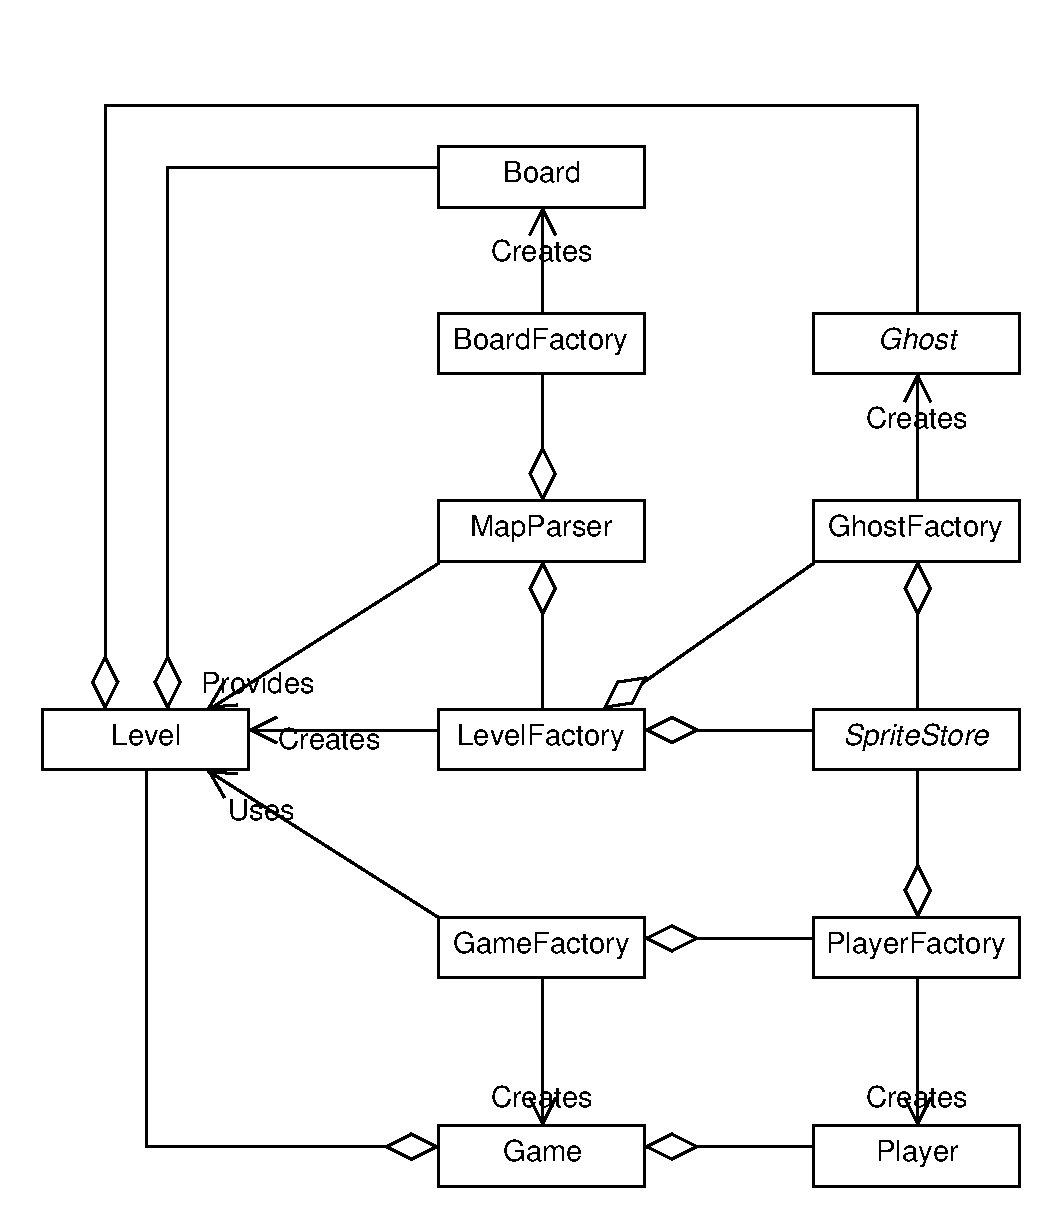
\includegraphics[scale=0.4]{imgs/FactoryWiring.pdf}
    \caption{Factory Wiring Class Diagram}
    \label{fig:FactoryWiringClassDiagram}
\end{figure}

\begin{figure}[h]
    \centering
    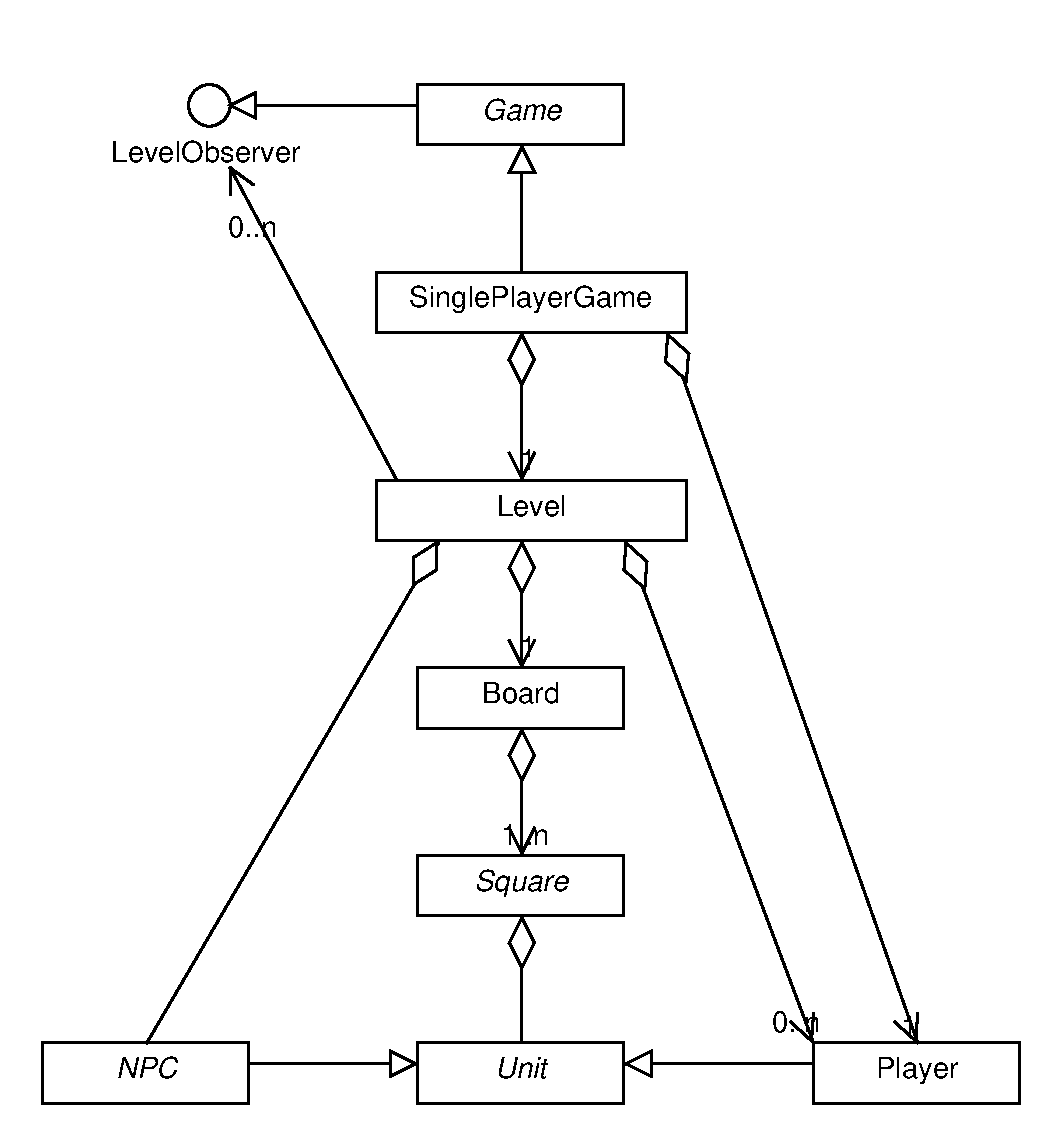
\includegraphics[scale=0.4]{imgs/SinglePlayerGame.pdf}
    \caption{Single Player Game Class Diagram}
    \label{fig:SinglePlayerGameClassDiagram}
\end{figure}

\subsubsection{Static Analysis}

\paragraph{Bad Smells (Designite)}

Designite is a code analyzer which can detect bad smells in a project. Firstly, made for C\# implementation, another version for Java project is provided. Here, designite is used as an \textit{IntelliJ} plugin to have a live visualization during the refactoring and as a "script" to get global information from the project as \textit{csv} files (sample of used file see Table ~\ref{tab:BadSmells}). Furthermore, the output of the "script" gives some information (see Figure ~\ref{fig:DesigniteOutput}), such as the number of cyclic dependency, here 5, the number of magic number, here 39 and also the number of long parameter list, here 8. \\


\begin{table}[h]
    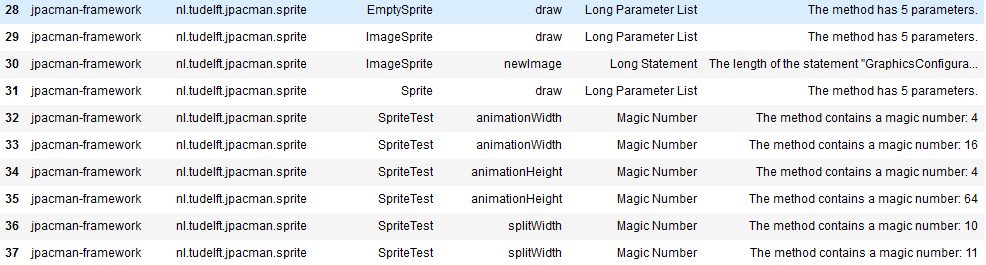
\includegraphics[scale=0.5]{imgs/badSmellsSample.PNG}
    \caption{ImplementationSmells.csv}
    \label{tab:BadSmells}
\end{table}

\begin{figure}
    \centering
    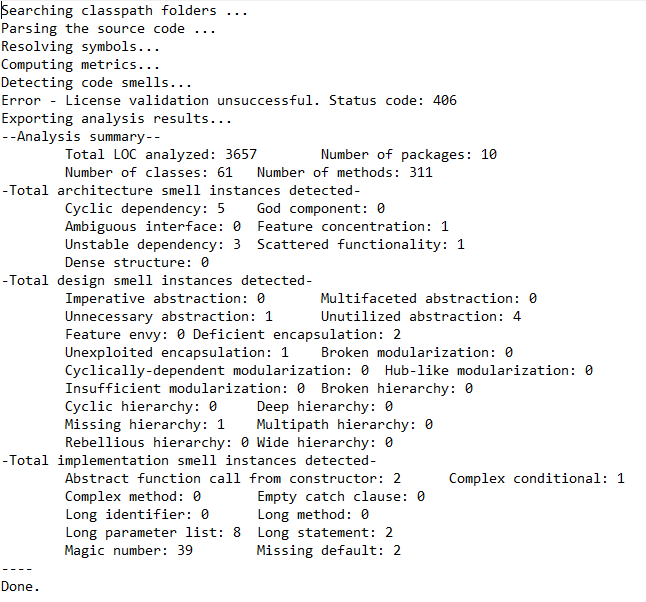
\includegraphics[scale=0.6]{imgs/DesigniteOutput.PNG}
    \caption{Designite Output}
    \label{fig:DesigniteOutput}
\end{figure}

\paragraph{Code Metrics (CodeMR)}

CodeMR is a software which assess a project quality with a static code analysis to help developers or companies to develop better code, products quality. It generates an interactive \textit{html} files to visualize all information assessed as a dashboard.\\

The main page (see Figure ~\ref{fig:CodeMRDashboard}) informs that the project quality is fairly good. Only one problematic class and $9.9\%$ of cohesion lack. \\

By coupling the Figures ~\ref{fig:CodeMRByPackage} and ~\ref{fig:CodeMRDashboard}, we notice that the class \textit{Level} impacts the project quality. The problematic metric, visible from the Figure ~\ref{fig:CodeMRLevelClassQuality}, is the lack of cohesion\footnote{https://www.codemr.co.uk/documents/} defined in the \textit{CodeMR} as "Measure how well the methods of a class are related to each other. High cohesion (low lack of cohesion) tend to be preferable, because high cohesion is associated with several desirable traits of software including robustness, reliability, reusability, and understandability. In contrast, low cohesion is associated with undesirable traits such as being difficult to maintain, test, reuse, or even understand.".

\begin{figure}
    \centering
    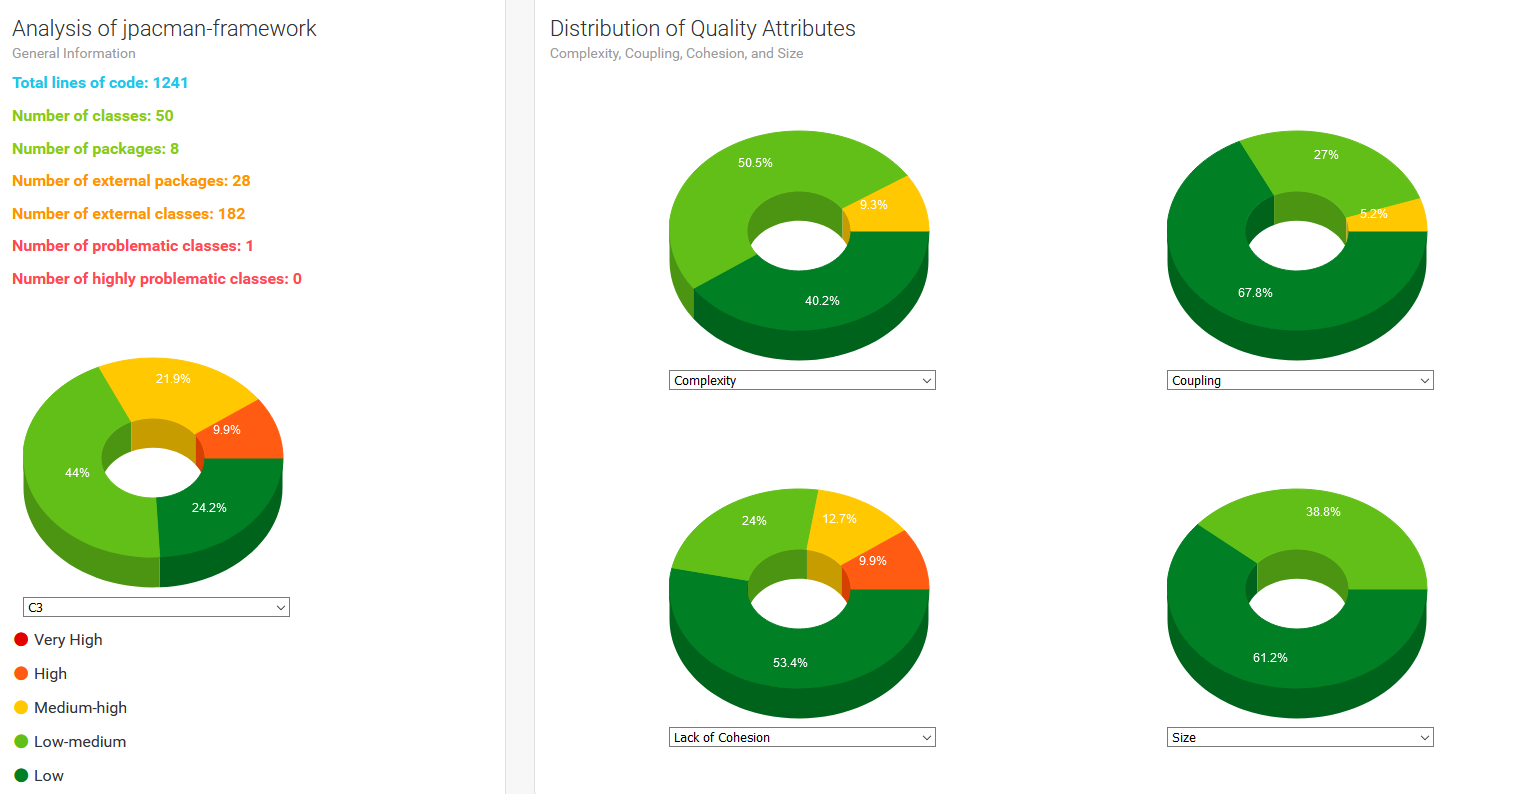
\includegraphics[width=\linewidth]{imgs/CodeMRDashboard.PNG}
    \caption{CodeMR dashboard summarizing health of the system 1}
    \label{fig:CodeMRDashboard}
\end{figure}

\begin{figure}
    \centering
    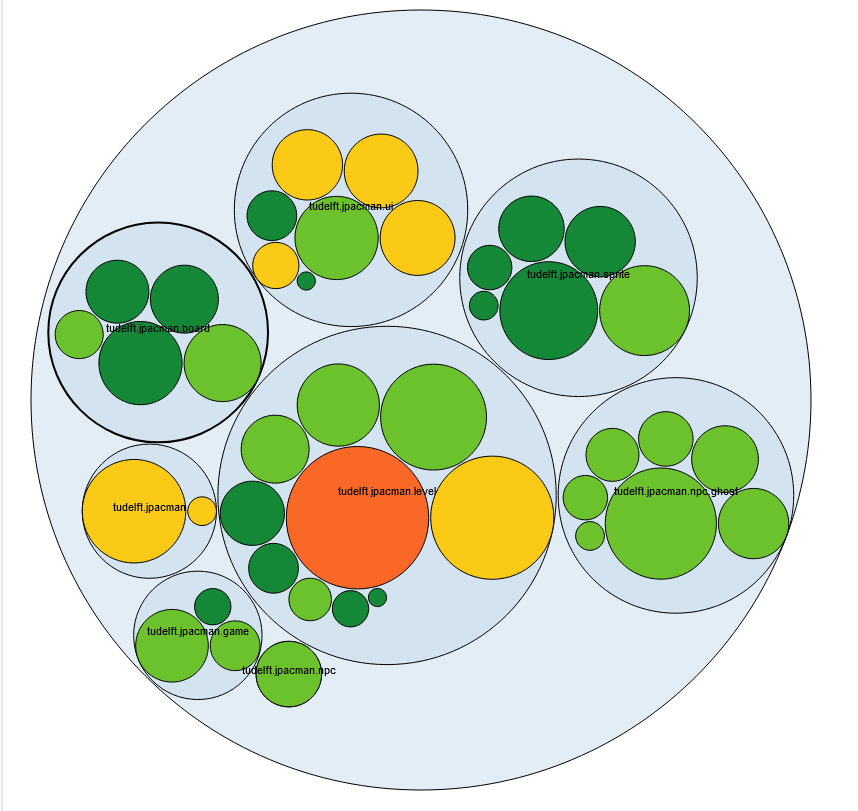
\includegraphics[scale=0.5]{imgs/CodeMRByPackage.PNG}
    \caption{C3 Metric by package for the system 1}
    \label{fig:CodeMRByPackage}
\end{figure}

\begin{figure}
    \centering
    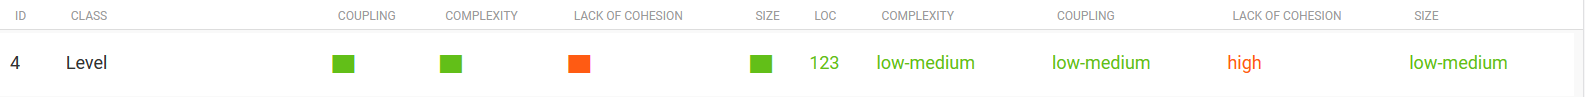
\includegraphics[width=\linewidth]{imgs/CodeMRLevelMetrics.PNG}
    \caption{Metrics of the class Level}
    \label{fig:CodeMRLevelClassQuality}
\end{figure}

\paragraph{Dependencies (IntelliJ analyzer)}

IntelliJ Ultimate version has an analyzer to assess a dependencies matrix (see Figure ~\ref{fig:DependenciesMatrixS1}). We observe, as seen before with Designite analysis, few cyclic dependencies.

\begin{figure}
    \centering
    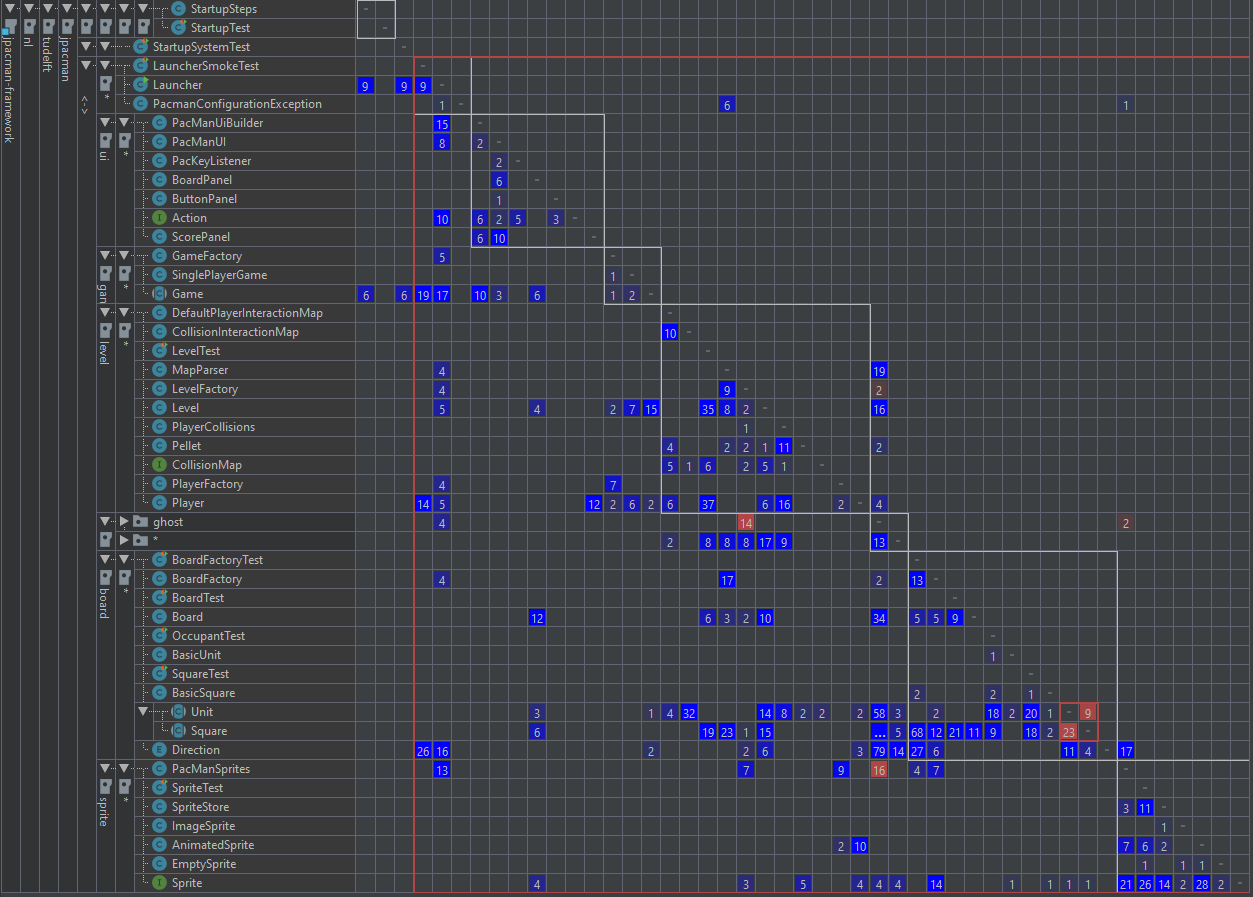
\includegraphics[width=\linewidth]{imgs/matrix dependencies.PNG}
    \caption{Matrix of Dependencies}
    \label{fig:DependenciesMatrixS1}
\end{figure}

\paragraph{Javadoc Coverage (MetricsReloaded)}

With the plugin \textit{MetricsReloaded} of \textit{IntelliJ}, we can assess few metrics like the Javadoc coverage (see Figure ~\ref{tab:javadocCoverageS1}). We observe that the project is fairly covered by the javadoc.

\begin{table}
    \centering
    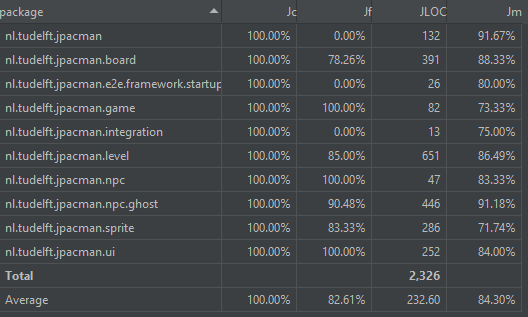
\includegraphics[width=\linewidth]{imgs/JavaDocCoverageS1.PNG}
    \caption{Coverage of the javadoc for the system 1}
    \label{tab:javadocCoverageS1}
\end{table}

\subsubsection{Dynamic Analysis}

\paragraph{Running tests \& Test Coverage (IntelliJ Build-Run)}

By running the tests provided with the project, 45 of 45 tests passed. Furthermore, IntelliJ provides a tool to assess the coverage of tests (see Table ~\ref{tab:TestCoverageS1}). Looking at the \textit{Method, \%} column, it's fairly well covered. We see that the Package \textit{level} is covered at 66\%. \\

In the Table ~\ref{tab:TestCoverage2S1}, we get more detailed information and observe that two classes are not tested, \textit{CollisionInteractionMap} and \textit{DefaultPlayerInteractionmap}. Furthermore, another class, \textit{LevelFactory} is covered at 50\%. Some enhancement can be done for it.

\begin{table}
    \centering
    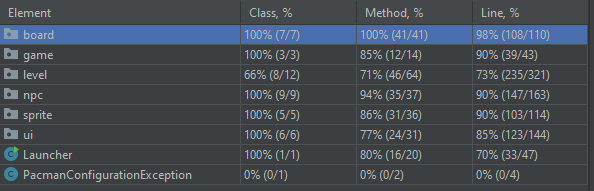
\includegraphics[width=\linewidth]{imgs/testCoverageS1.PNG}
    \caption{Test Coverage for the system 1}
    \label{tab:TestCoverageS1}
\end{table}

\begin{table}
    \centering
    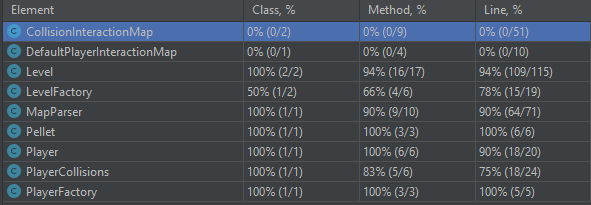
\includegraphics[width=\linewidth]{imgs/testCoverage2S1.PNG}
    \caption{Test Coverage Package level for the system 1}
    \label{tab:TestCoverage2S1}
\end{table}

\newpage

\section{Quality improvement}

\subsection{System 1 (BOOSKO Sam)}

In general, the provided implementation didn't need improvement but few were done like making an object as a parameters for method with too many parameters. Furthermore, few magic numbers were fixed in unit test implementation. Mainly, magic numbers were in testing codes, then it's normal to have them there. It's more readable to understand them and write them.\\

The part of the implementation in \textit{MapParser} which manage the creation of element of the game from a text file were modify to increase the readability and help new developers to add new elements in the project. At first, it was done with a switch case on a \textit{Char}. To make it more modular, an Interface, called \textit{ISquareBuilder}, was create. This class take as parameter and object, \textit{AddSquareParameters}, which contains all information of the game to create easily and new element. An abstract class, \textit{ADefaultSquareBuilder}, implementing this interface, is also created. This abstract class helps to reduce the duplication code. Finally, it's pretty easy to add a new element on the grid by adding the \textit{Char} key and the responding ISquareBuilder. \\

\section{Adding basic functionalities}

\subsection{System 1 (BOOSKO Sam)}

The provided project missed basic functionalities, such as the continuous PacMan Moving, fruit elements, power pellet...\\

The first feature added is the continuous PacMan moving, a new class is created for ot, \textit{PlayerController}. This class contains information from the game and have a scheduled action. This action is simply to move the pacman to the register position. This direction can be changed by a key listener. The speed of the pacman is managed here with two attributes, 1) $Speed$ and 2) $SpeedModifier$. With them, the final speed is compute as $speed * speedModifier$. Where the speed unit is the number of tiles per second. The speed modifier is thought to help the implementation of extensions.\\

Secondly, to be able to add new elements that pacman can eat on the board, the class \textit{Pellet} is edited to add an action \textit{onEat(Level level, Player player)} where the player is the pacman who ate the element. This action is called when a player have a collision with a pellet element. With this method, it was easy to implement the feature of scared ghosts (Pacman can eat a scared ghost) and the feature of new life by eating fruits.\\

Everything was thought to help another person to add new features from the sectioned extension. Adding a new element on the board take $1$ minute. The longest time being the implementation of the action performed of this new element.\\

\section{Adding new features}

\subsection{System 3 (BOOSKO Sam)}

\subsubsection{Quality Improvement}

The title sounds weird in this section because we had to improve the quality in the previous step. Unfortunately for me, after reading the implementation and listening Robin speech about his work, I could notice that, it wouldn't be easy to add easily new features as demanded. I decided to rework few part of the system 3 based on what I did and saw in System 1.\\

Firstly, I changed the method based on a \textit{switch-case} in an object which creates a game element from a \textit{character} by a \textit{HashMap} where the keys are a \textit{Character} and the value an object, \textit{IElementBuilder}. The same way is used to create \textit{Cell} of the board. It's useful to bridge because bridges are not a game element but cell.\\

Secondly, I implemented a new object to manage collision with my new game element. Because, it wasn't my job to rework this system. I didn't change the previous collision detection. I added mine just to manage new collisions. It's based on a double \textit{HashMap} accesible by a couple of key (\textit{Class object}) to get an \textit{ICollisionAction} to perform the action on the game from this collision. \\

Finally, the last reworking is on \textit{MovingGameElement}. This class doesn't have any documentation and have an attribute \textit{speed}. It's quite difficult to understand the unit used for the speed and very diffult to \texttt{play} with it. Then, I decide to modify it to have a speed based on the unit, such as the number of cells traveled per second because usually, the speed unity follows the format such as $x$ unit of distance per $t$ unit of time. Also deleting code duplication from \textit{Pacman class} and \textit{Ghost class}, both extending \textit{MovingGameElement}.\\

\subsubsection{Features}

To be able to add new game element, a new abstract class is created, \textit{AExtensionElement}. This class provides a simply implementation to display an image for this game element. Also, to use this class such as a game element, it extends the main class \textit{GameElement}. Another little feature is the possibility to change the Pacman color to have a visualisation about his state.\\

\paragraph{Traps}

When Pacman goes on this game element, he is trapped for a random time between 1 and 4 seconds and turns red. This feature is implemented in \textit{pacman\_infd.Elements.ExtensionElements.TrapElement} (see Figure ~\ref{fig:system3Traps}).\\

\begin{figure}
\centering
    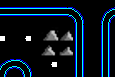
\includegraphics[width=.4\linewidth]{imgs/trapbefore.PNG}
    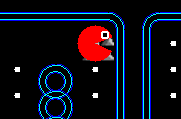
\includegraphics[width=.4\linewidth]{imgs/trapafter.PNG}
    \caption{System 3 - Traps}
    \label{fig:system3Traps}
\end{figure}

\paragraph{Teleportation} This game element is working by couple, because when the Pacman use a portal, he needs the output of this portal. In the rule chosen, only two portals can be created on a board. Also, a timer is used after the usage of a portal making the link broken during 2 seconds (see ~\ref{fig:system3Portals}). This feature is implemented in \textit{pacman\_infd.Elements.ExtensionElements.TeleporterElement}. 

\begin{figure}
\centering
    
\includegraphics[width=.3\linewidth]{imgs/portal1.PNG}
    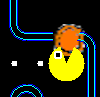
\includegraphics[width=.3\linewidth]{imgs/portal2.PNG}
    \caption{System 3 - Portals}
    \label{fig:system3Portals}
\end{figure}

\paragraph{Bridges} The bridges was the most complex feature to implement because it's not considered as a game element in this System. The best way to make this feature is to create a new kind of \textit{Cell}. This special cell assesses where is the \textit{MovingGameElement}, under or above the bridge. From this, it requires an override of default methods from \textit{Cell}. Two new lists are used, one with \textit{MovingGameElement} under the bridge and another one with \textit{MovingGameElement} above the bridge. Also, updates are made on the \textit{EventHandler} to let the collision checking assessing in the Cell object and on the \textit{MovingGameElement} to be able to know the current direction of the element. Thanks to these updates, the new Cell kind can manage how it wants the collision between game elements on itself and assesses as said where is the game element depending on his direction. This feature is mainly implemented in \textit{pacman\_infd.Game.BridgeCell} (see ~\ref{fig:system3Bridge}).

\begin{figure}
\centering
    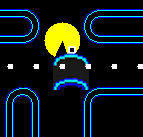
\includegraphics[width=.3\linewidth]{imgs/bridge1.PNG}
    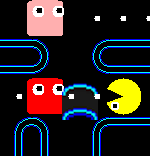
\includegraphics[width=.3\linewidth]{imgs/bridge2.PNG}
    \caption{System 3 - Bridges}
    \label{fig:system3Bridge}
\end{figure}

\paragraph{Grenade} The Grenade is implemented in \textit{pacman\_infd.Elements.ExtensionEle\\ments.GrenadeElement}. In the rule chose, the grenade kills all ghosts around in the maximum distance of 4 cases with a special specification. The grenade doesn't cross the walls. It means that a ghost can survive if he is protected by a wall. The main method for this is implemented on \textit{Cell} where a \textit{Breadth First Search} is implemented. The method takes two parameters, the Class (extends GameElement) searched in a maximum distance given as the second parameter (see ~\ref{fig:system3Grenade}.

\begin{figure}
\centering
    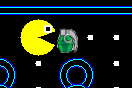
\includegraphics[width=.4\linewidth]{imgs/grenadeBoard.PNG}
    \caption{System 3 - Grenades}
    \label{fig:system3Grenade}
\end{figure}

\paragraph{Red Beans} The Red Bean, implemented in \textit{pacman\_infd.Elements.Extension\\Elements.RedBeanElement}, is a special element. When Pacman eats this bean, Pacman is slown down by 50\% but he shoots 3 projectiles per second. These projectiles have the speed of $Pacman + 10$. Also, Pacman turns in dark red. The \textit{MovingGameElement} is used to create these projectile easily and a new collision is added in the \textit{CollisionMap} between \textit{Ghost} and \textit{Projectile} (see Figure ~\ref{fig:system3RedBeans}).

\begin{figure}
\centering
    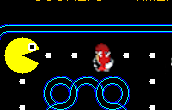
\includegraphics[width=.3\linewidth]{imgs/redBeanElement1.PNG}
    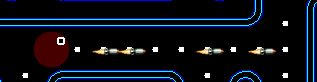
\includegraphics[width=.6\linewidth]{imgs/redBeanElement2.PNG}
    \caption{System 3 - Red Beans}
    \label{fig:system3RedBeans}
\end{figure}

\paragraph{Potato} The Potato, implemented in \textit{pacman\_infd.Elements.ExtensionElement\\s.PotatoElement}, is a a simple element which increase the speed of all ghost on the board by 2 during a time. For this element, the visual information is done by ghosts which are faster than Pacman (see Figure ~\ref{fig:system3Potato}).

\begin{figure}
\centering
    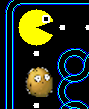
\includegraphics[width=.3\linewidth]{imgs/potato.PNG}
    \caption{System 3 - Potato}
    \label{fig:system3Potato}
\end{figure}

\paragraph{Fish} The fish is another simple element and the last, this one, implemented in \textit{pacman\_infd.Elements.ExtensionElements.PotatoElement}, slows down the Pacman to a very slow speed and he turns cyan (see Figure ~\ref{fig:system3Fish}) . 

\begin{figure}
\centering
    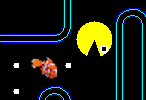
\includegraphics[width=.3\linewidth]{imgs/fish1.PNG}
    
\includegraphics[width=.3\linewidth]{imgs/fish2.PNG}
    \caption{System 3 - Fish}
    \label{fig:system3Fish}
\end{figure}

\paragraph{Elements Spawning System} All elements can be setup in the file map. During the game, two elements, the bridges and the teleporters don't spawn by the spawning system. This spawning system works such as for each pellet ate, there is 10\% that a random elements spawn on an empty \textit{cell}. This system is implement in the object \textit{GameWorld} on the method \textit{placeCherryOnRandomEmptyCell} already provided.

\section{Quality evolution analysis}

\subsection{System 3 (BOOSKO Sam)}

\subsubsection{Generalities}

The personal view is that a lot of improvements can be done, but it should mean, rework all the system. This system, is, according to me, not good. A lot of parts are not clear, not easy to modify, or to update without changing a huge part of it. It would be too long to enumerate all of these problems seen. But few of them are, 1) the merging between, the controller, the visual and the core (model), 2) using not logical value for attributes as the previous speed in the object \textit{MovingGameElement}, increasing this value gave the effect of slowing down the GameElement, 3) the class \textit{Wall}, don't need to explain, just opening it make us understand and many more problems could be said.\\

\subsubsection{Static Analysis}

\paragraph{Bad smells (Designite)} 
With Designite, we observe that there are 229 magic numbers (see Figure ~\ref{fig:system3EndStepDesignite}), corresponding in the implemention of the default elements drawing method. In general, the system is doing well. 

\begin{figure}
\centering
    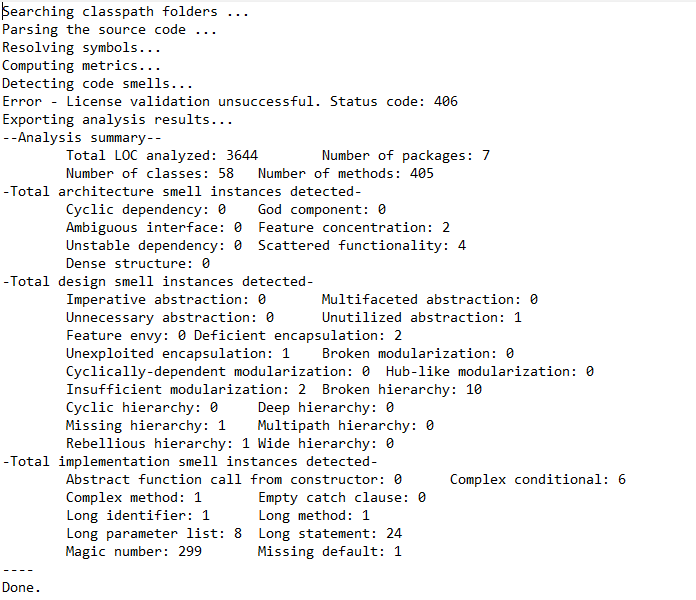
\includegraphics[width=\linewidth]{imgs/system3LastStepDesignite.PNG}
    \caption{System 3 - Designite Output}
    \label{fig:system3EndStepDesignite}
\end{figure}

\paragraph{Javadoc Coverage (MetricsReloaded)}
We observe that the javadoc coverage should be improved (see Table ~\ref{tab:system3EndStepJavaDoc}).

\begin{table}
\centering
    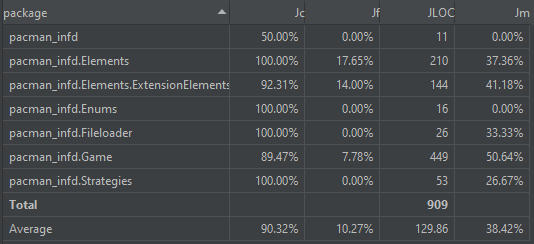
\includegraphics[width=\linewidth]{imgs/JavaDocCoverageS3.PNG}
    \caption{System 3 - Javadoc Coverage}
    \label{tab:system3EndStepJavaDoc}
\end{table}

\subsubsection{Dynamic Analysis}

\paragraph{Running tests \& Test Coverage (IntelliJ Build-Run)} By running the tests provided and new tests added, 28 tests of 28 passed. Furthermore, the project is quite well covered by tests (see Table ~\ref{tab:system3EndStepTestCoverage}). Anyway, some improvements could be done.

\begin{table}
\centering
    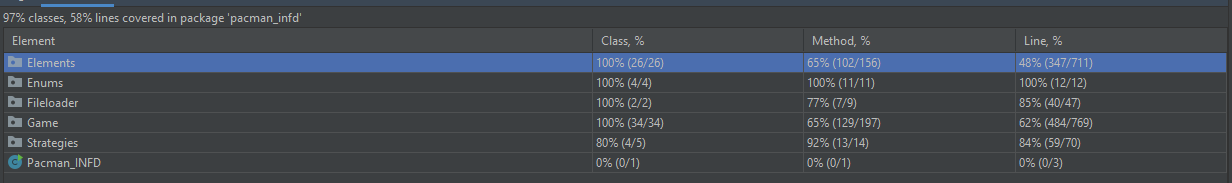
\includegraphics[width=\linewidth]{imgs/system3lastStepTestCover.PNG}
    \caption{System 3 - Test Coverage}
    \label{tab:system3EndStepTestCoverage}
\end{table}

\section{Conclusion}

\end{document}
